\section{Design}
\label{sec:design}
This section will explain how both tasks A and B will be completed, giving diagrams and flowcharts of how the E-Pucks will carry out a particular task.
\subsection{Task A}
To begin designing a solution to the tasks set out in section \ref{sec:intro}, one must first decide upon the different behaviours to be implemented for the tasks. A relatively simple task to be implemented, which would be beneficial to both the first and second task, would be to implement a love behaviour.

Section \ref{sec:background} discussed how each behaviour would perform, illustrating that the love behaviour would follow but not touch the leading object. A second behaviour to be implemented would be an adaption of the aforementioned love behaviour, although instead of the E-Puck following an object it would instead follow a bright light placed before it. The E-Puck would use both the camera to discover any spots of light that have a much higher intensity than its surroundings.

One third and final possible behaviour to implement, providing time permits the group to do so, would be to to implement a obstacle avoidance behaviour. The behaviour which attempts to avoid any nearby objects whilst moving in a particular direction. When it approaches an object it changes its direction to move away from the object.

The first and final behaviours rely heavily on the infrared senses situated on around the edge of the E-Puck. The E-Puck will read in from the infrared sensors, each returning a voltage reading to the chip. This reading can then be used within a formula to calculate the distances to a nearby object. When an object is discovered nearby, the E-Puck must either turn to face it or alter it's direction to move away from it, for the love and obstacle avoidance behaviours respectively. The E-Puck is then required to move forward at a fixed speed until either the object is very close, but not touching for the love behaviour or no longer detected for the hate behaviour.

To create the second behaviour of an attraction to light the E-Puck must be implemented in a similar way to the previously mentioned behaviours, although instead of reading the infrared sensor value for distance one will measure the amount of ambient light falling onto the device.

\subsection{Task B}
Task B requires the group to implement 2 different E-Pucks and cause each to do their own tasks. One E-Puck will be required to follow a hand whilst the other E-Puck will be required to follow the first E-Puck. This may seem similar after implementing the behaviours from task A, although many issues could arise with this task. These issues will be discussed toward the end of this section.

Since the love behaviour will have already been implemented once the implementation of task B begins it would be logical to make use of these behaviours to save time. Therefore to obtain the the desired output of the second E-Puck (the following of the first E-Puck), one may use this behaviour and achieve the required result.

For the first E-Puck, the E-Puck which will be following a human hand, the group will have to use both the camera and infrared sensors on the E-Puck and consult the research performed within section \ref{sec:background} surrounding the colour of human skin.

The E-Puck will begin by discovering any near-by objects using the infra-red sensors before turning the front camera towards any discovered objects. The front camera will then read in the image of the object. Removing a few rows of pixels from the image, for fast processing, the pixels will then be processed to find any required colour that the E-Puck is looking for, the colour of a hand. This processing will be done in the HSV colour plane as to reduce the impact lighting has on the colour of an image.

\subsubsection{Flowchart}
\begin{figure}
	\centering
	\captionsetup[subfigure]{justification=centering}
	\begin{subfigure}{0.45\textwidth}
		\centering
		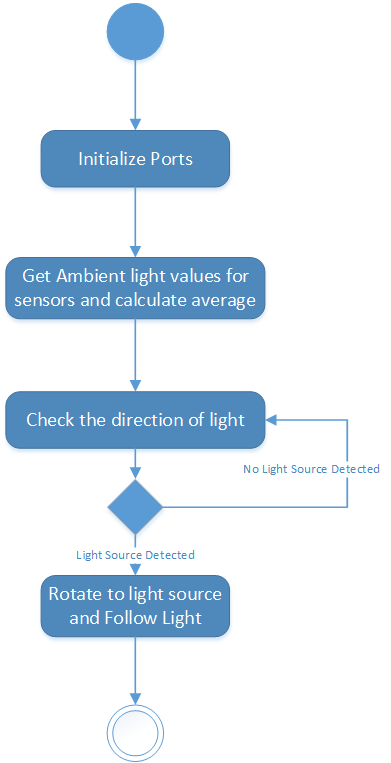
\includegraphics[width=0.5\textwidth]{figures/FollowLight.png}
		\label{fig:flowFollowLight}
		\caption{Flow chart describing \\ the follow light function}
	\end{subfigure}
	\begin{subfigure}{0.45\textwidth}
		\centering
		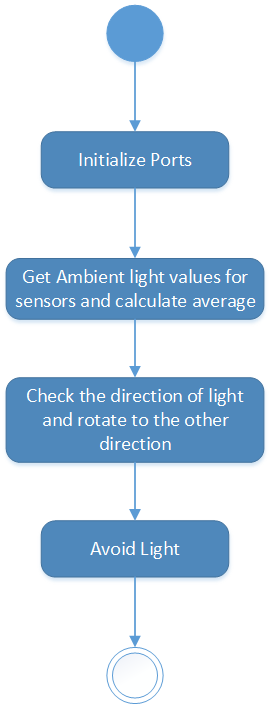
\includegraphics[width=0.5\textwidth]{figures/AvoidLight.png}
		\label{fig:flowAvoidLight}
		\caption{Flow chart describing \\ the avoid light function}
	\end{subfigure}
	\begin{subfigure}{0.9\textwidth}
		\centering
		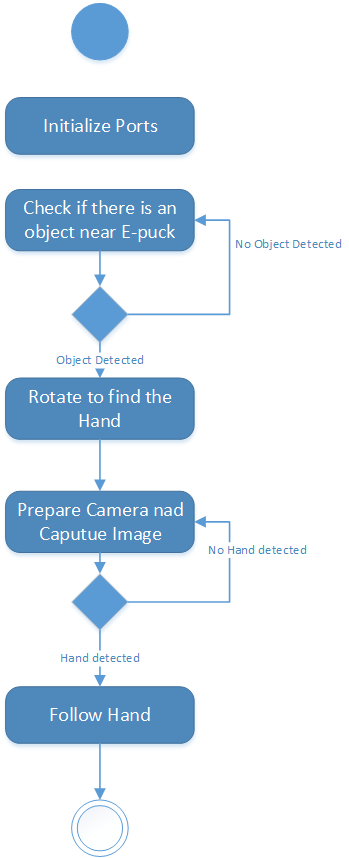
\includegraphics[width=0.3\textwidth]{figures/FollowHand.png}
		\label{fig:flowFollowHand}
		\caption{Flow chart describing \\ the follow hand function}
	\end{subfigure}
\caption{Flow charts describing 3 of the different behaviours implemented within the E-Puck}
\label{fig:flowBehav}
\end{figure}

\begin{figure}
\centering
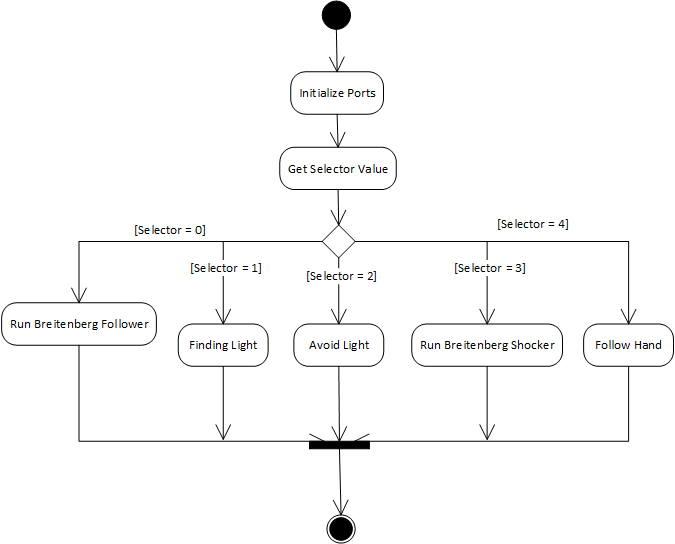
\includegraphics{figures/Main.png}
\caption{Flow chart describing how the main function will be implemented}
\label{fig:flowMain}
\end{figure}
